\documentclass[11pt]{report}
\renewcommand{\baselinestretch}{1.5}


% Declaração dos pacotes
\usepackage[utf8]{inputenc}
\usepackage[T1]{fontenc}
\usepackage{graphicx}
\usepackage[portuguese]{babel}
\usepackage{graphicx}
\usepackage[affil-it]{authblk} % Usado para meter nome da escola
\usepackage{eurosym} % Usado para o €
\usepackage{url} % URL



% CAPA
\title{\textbf{\textit{Exploração e desenvolvimento  de processos de interoperabilidade entre sistemas, assentes em serviços web.}\\
		\large2º Trabalho prático de
		Integração de Sistemas de Informação}}
			
				
\author{Rúben Guimarães nº11156}

\affil{Escola Superior de Tecnologia, IPCA \\
	Barcelos}	
	
		
\date{10 de Novembro de 2017}


\begin{document}

\maketitle




% Indice
\tableofcontents


% Introdução
\chapter*{Introdução}
\addcontentsline{toc}{chapter}{Introdução}

O trabalho prático abordado neste relatório foi desenvolvido no âmbito da unidade curricular Integração de Sistemas de Informação do curso de Engenharia de Sistemas Informáticos, lecionada pelo docente Luís Ferreira. O docente desafiou os alunos a criar um projeto que aplicasse e experimenta-se serviços SOAP e RESTful, complementada com a utilização de serviços externos existentes.

\clearpage



% Resumo
\chapter*{Resumo}
\addcontentsline{toc}{chapter}{Resumo}

Neste trabalho desenvolvi um pequeno serviço que é alojado na platforma Azure que é uma solução para alojamento de serviços e aplicações na \textit{cloud}. 
Este serviço recorre a 4 API's externas para receber informação sobre o endereço IP da nossa ligação ou de uma fornecida, para recolher informação metereologica de uma dada cidade e por fim para publicar um \textit{Tweet} no \textit{Twitter} ou para publicar a informação metereologica da cidade consultada no \textit{Twitter}.\\ Por fim desenvolvi recorrendo ao \textit{Windows Presentation Foundation} (WPF) que recorre a linguagem de marcação \textit{Extensible Application Markup Language} (XAML) um cliente que utiliza os serviços desenvolvidos.

\clearpage


% Objectivos
\chapter*{Objectivos}
\addcontentsline{toc}{chapter}{Objectivos}

Os objetivos que defini para o meu projeto foram os seguintes:

\begin{itemize}
\item Usar uma API externa para saber o endereço IP da minha ligação.
\item Usar uma API externa para saber informação sobre um endereço IP.
\item Usar uma API externa para publicar \textit{Tweets} no \textit{Twitter}.
\item Usar uma API externa para receber informação metereologica de uma cidade.
\item Controlar a execução de serviços com recurso a credencias de autenticação (protocolo OAuth).
\item Publicar o serviço na platforma Azure.
\item Publicar e usar uma base da dados na platforma Azure.
\item Desevolvimento de um cliente que utilize os serviços desevolvidos.
\item Diversos tipo de operações CRUD recorrendo aos serviços RESTful.
\item Utilização de um sistema de controlo de versões no desevolvimento (GIT).
\end{itemize}


\clearpage


% Arquitectura
\chapter*{Arquitectura}
\addcontentsline{toc}{chapter}{Arquitectura}

Podemos consultar na figura seguinte um diagrama com a arquitectura do projecto.

\begin{figure} [!h]
\centering
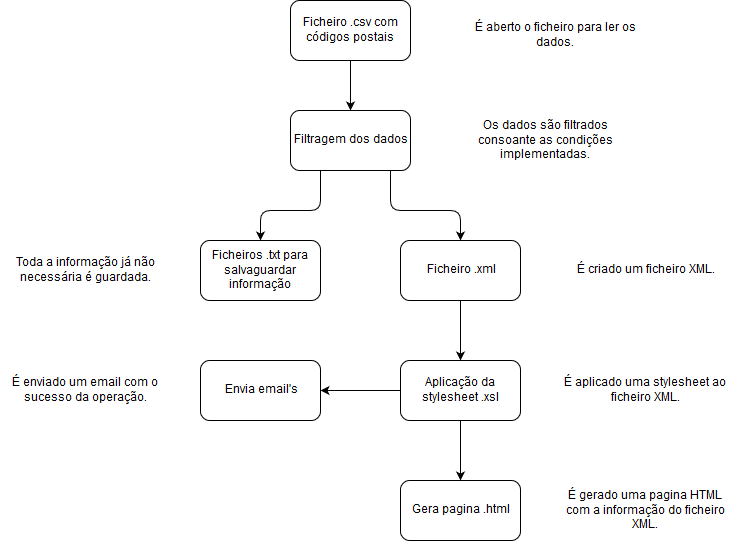
\includegraphics[width=\textwidth]{Prints_Trabalho/diagrama}
\caption{Diagrama da arquitectura do projecto}
\label{Rotulo}
\end{figure}


\clearpage


% Principais Passos
\chapter*{Principais momentos ETL}
\addcontentsline{toc}{chapter}{Principais momentos ETL}

O primeiro passo começa com o inicio do c no Pentaho, este cria uma nova pasta para guardar os ficheiros criados e começa o processo de \textit{transformation}.\\
O processo de \textit{transformation} começa por carregar o ficheiro com os dados dos codigos postais.


\begin{figure} [!h]
\centering
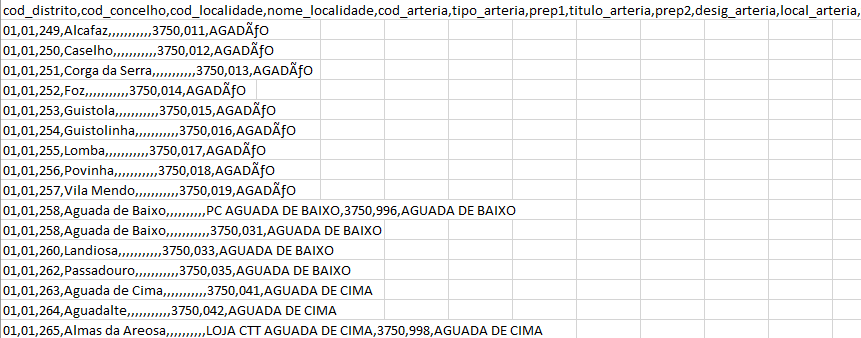
\includegraphics[width=\textwidth]{Prints_Trabalho/excel}
\caption{Extracto do ficheiro com os dados}
\label{excel}
\end{figure}


\clearpage

Os dados são filtrados quer por expressões regulares quer pelo nome da freguesia. Os dados que já não forem necessarios são guardados em ficheiros .txt.

\begin{figure} [!h]
\centering
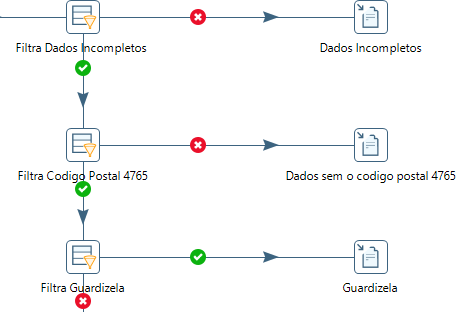
\includegraphics[width=\textwidth]{Prints_Trabalho/filtra}
\caption{Parte da filtragem no processo de \textit{transformation} no Pentaho}
\label{filtragem}
\end{figure}

De seguida os nome das ruas são concatenados e é gerado um ficheiro XML.

\begin{figure} [!h]
\centering
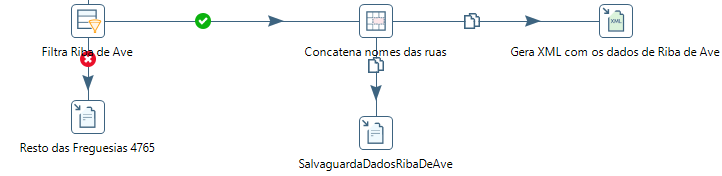
\includegraphics[width=\textwidth]{Prints_Trabalho/concatena}
\caption{Contatenação do nome das ruas e criação do ficheiro XML}
\label{xml}
\end{figure}

O proximo passo é a aplicação da stylesheet ao ficheiro XML.

\begin{figure} [!h]
\centering
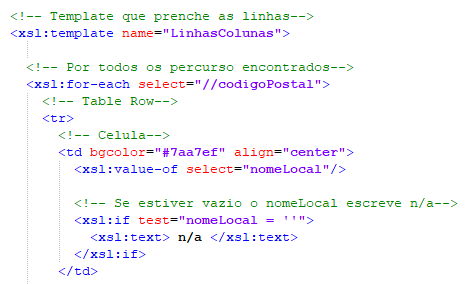
\includegraphics[width=\textwidth]{Prints_Trabalho/xsl}
\caption{Extracto do ficheiro XSL}
\label{xsl}
\end{figure}

Por ultimo é enviado um email com o sucesso/insucesso da operação.

\begin{figure} [!h]
\centering
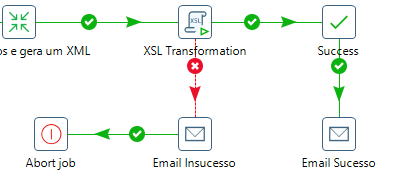
\includegraphics[width=\textwidth]{Prints_Trabalho/mail}
\caption{Flow de envio do email}
\label{mail}
\end{figure}




\clearpage





% Conclução
\chapter*{Conclusão}
\addcontentsline{toc}{chapter}{Conclusão}

Este trabalho permitiu-se aplicar os conhecimentos adquiridos durante o desenrolar da unidade curricular de Integração de Sistemas de Informação e explorar novos conceitos de ETL. Se tivesse mais tempo gostaria de ter implementado o uso de um serviço Web, que adiciona-se as coordenadas da rua ao ficheiro XML e ter criado ficheiros XML para todas as freguesias.

% Bilbiografia
\begin{thebibliography}{2}
	\bibitem{central_dados}
	Transparência Hackday Portugal. \emph{Central de Dados}.  08 Novembro, 2017. 
	\url{http://centraldedados.pt/codigos_postais/}
	

\end{thebibliography}
\addcontentsline{toc}{chapter}{Bibliografia}

\end{document}